%%%%%%%%%%%%%%%%%%%%%%%%%%%%%%%%%%%%%%%%%%%%%%%%%%%%%%%%%%%%%%%%%%%%%
% University Assignment Title Page 
% LaTeX Template
% Version 1.0 (27/12/12)
%
% This template has been downloaded from:
% http://www.LaTeXTemplates.com
%
% Original author:
% WikiBooks (http://en.wikibooks.org/wiki/LaTeX/Title_Creation)
%
% License:
% CC BY-NC-SA 3.0 (http://creativecommons.org/licenses/by-nc-sa/3.0/)
%%%%%%%%%%%%%%%%%%%%%%%%%%%%%%%%%%%%%%%%%%%%%%%%%%%%%%%%%%%%%%%%%%%%%

\documentclass[11pt,canadien]{article}

\usepackage{babel} % Pour la typo canadienne
\usepackage{graphviz} % Pour inclure des images
\usepackage[utf8]{inputenc} % Pour les accents sur le document
\usepackage{mathptmx} % Pour Times New Roman
\usepackage[top=1in,bottom=1in,left=1in,right=1in]{geometry} % Marges de 1 pouce
\usepackage[toc,page]{appendix} % Pour avoir des annexes et qui figures sur le sommaire

\begin{document}

\begin{titlepage}

\newcommand{\HRule}{\rule{\linewidth}{0.5mm}} % Defines a new command for the horizontal lines, change thickness here

\center % Center everything on the page
 
%-----------------
% HEADING SECTIONS
%-----------------


\includegraphics[width=\textwidth]{images/uqac_logo.jpg} % logo
 
\textsc{\LARGE 8IFG145 - Gestion de projets informatique}\\[0.5cm]

%--------------
% TITLE SECTION
%--------------

\HRule \\[0.4cm]
{ \huge \bfseries TP1 - Compréhension et exécution de commandes avec GitHub}\\[0.4cm]
\HRule \\[0.5cm]
 
%---------------
% AUTHOR SECTION
%---------------

\begin{minipage}{0.4\textwidth}
\begin{flushleft} \large
\emph{Étudiants :}\\
Antoine \textsc{Moreau}\\
Estelle \textsc{Michel}\\
Joffrey \textsc{Germain}\\
Julien \textsc{Naty}\\
Karen \textsc{Migan}\\
Kévin \textsc{Seroux}\\
Valentin \textsc{Tertois}\\
\end{flushleft}
\end{minipage}
~
\begin{minipage}{0.4\textwidth}
\begin{flushright} \large
\emph{Professeur :}\\
Dany \textsc{Fortin-Simard}
\end{flushright}
\end{minipage}\\[2cm]

%-------------
% DATE SECTION
%-------------

{\large \today}\\[2cm]

\vfill % Fill the rest of the page with whitespace

\end{titlepage}

\newpage
\tableofcontents

\newpage
\section{Introduction au langage Git et à l'outil Github}
Blablabla

\newpage
\section{Apprentissage de Github}
Les commandes \texttt{merge}, \texttt{fetch}, \texttt{pull}, \texttt{push} prennent facultativement en argument le dépôt distant (ex: origin) et la branche distante (ex: master).

\paragraph{git commit}La commande \texttt{git commit} est une des commandes principales de l'outil git, elle permet de stocker le contenu de l'index et de "valider" les changements apportés aux fichiers présents dans le dépot. Habituellement, lors de
l'exécution de la commande, l'utilisateur utilise l'option \texttt{-m 'Mon texte'} afin de décrire les modifications apportés par cette nouvelle version des fichiers. 

\paragraph{git merge}Cette comamnde permet de fusionner deux branches. Cette commande va fusionner les commits des deux branches depuis leur séparation, le résultat de cette commande est qu'il ne restera plus qu'une branche, intégrant les
modifications apportées par les deux branches. L'option \texttt{-m 'Mon texte'} permet de préciser le message du commit qui sera effectué lors de la fusion des deux branches.

\paragraph{git cherry-pick}Cette commande permet d'appliquer les modifications d'un commit particulier d'une autre branche à la branche actuelle. Par exemple, si un correctif a été développé sur une autre branche, et qu'il devient nécessaire
de le déployer sur la branche principale, il est possible, grâce à \texttt{cherry-pick}, de ne récupérer que les modifications apportées par le commit qui nous intéresse.

\paragraph{git fetch}Mise à jour des références locales des branches distantes ainsi que des objets git (commit principalement). Dit autrement, elle permet au dépôt local, de prendre simplement conscience des modifications distantes. Elles ne sont pas appliquées aux branches locales. Cette commande est sûre.
\begin{figure}[h]
	\centering
	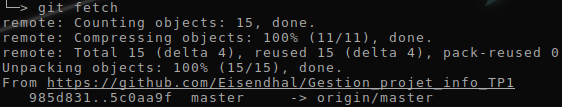
\includegraphics{images/git_fetch.png}
\end{figure}

\paragraph{git pull}Exécution d'un \texttt{git fetch} puis d'un \texttt{git merge}. Bien qu'elle soit pratique, quand la branche locale n'est pas derrière la branche distante, des fusions (avec commits parfois) sont effectués sans pouvoir annuler. Ce qui pose un soucis, pour la lisibilité de l'historique d'un dépôt. Il est d'usage d'utiliser plutôt \texttt{git pull --rebase} afin de remplacer l'opération de merging en une opération de rebasing. Il existe plusieurs façons par \texttt{git config} de spécifier ce comportement par défaut.
\begin{figure}[h]
	\centering
	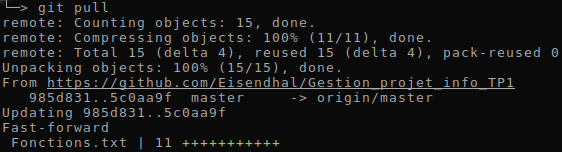
\includegraphics{images/git_pull.png}
\end{figure}

\paragraph{git push}Mise à jour des références du dépôt distant ainsi que des objets git (commit principalement). Dit autrement, elle permet au dépôt distant, d'appliquer les modifications locales. Il pourrait s'agir d'un git pull côté distant, sauf que c'est un autre dépôt qui est à l'initiative. Même si c'est rarement une bonne idée, on peut forcer le push si les branches locales et distantes ne sont pas cohérentes avec l'option \texttt{-f}.
\begin{figure}[h]
	\centering
	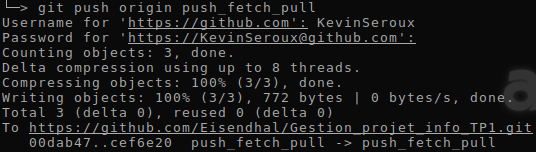
\includegraphics{images/git_push.png}
\end{figure}

%\paragraph{git status}la commande git-status permet d'afficher les chemins qui ont des differences entre le fichier index et le HEAD commit actuelle mais aussi les chemins qui ont des différences entre l'arbre actuelle et le fichier d'index et enfin les chemins l'abre actuel qui ne sont pas retenu par GIT. Les premiers chemins correspondent à ce que vous utiliseriez en faisent un git-commit tous les autre correspondent quand à eux à un git-add suivi d'un git-commit. L'option \texttt{-s] ou \texttt{--short} permet de formater l'affichage de la commande dans le format \texttt{short}.

\newpage
\section{Utilisation de Github}
Blablabla

\newpage
\begin{appendices} % Les annexes commencent

\section{Répartition des différentes tâches}
\begin{tabular}{l l l l}
	\textbf{Tâche} & \textbf{Temps} & \textbf{Date d'échéance} & \textbf{Responsable}
	\\ \hline
	   Partie 2 - Présentation de Git       & 3h    & 2016-09-15 & Antoine Moreau
	\\ Mise en forme du document final      & 3h    & 2016-10-04 & Kévin Seroux
	\\ Mise en place du dépôt Git et droits & 45min & 2016-09-08 & Joffrey Germain
	\\ Description \texttt{git add}         & 30min & 2016-09-15 & Estelle Michel
	\\ Description \texttt{git mv}          & 30min & 2016-09-15 & Estelle Michel
	\\ Description \texttt{git rm}          & 30min & 2016-09-15 & Estelle Michel
	\\ Description \texttt{git init}        & 30min & 2016-09-15 & Julien Naty
	\\ Description \texttt{git clone}       & 30min & 2016-09-15 & Julien Naty
	\\ Description \texttt{git rebase}      & 30min & 2016-09-15 & Julien Naty
	\\ Description \texttt{git status}      & 30min & 2016-09-15 & Valentin Tertois
	\\ Description \texttt{git log}         & 30min & 2016-09-15 & Valentin Tertois
	\\ Description \texttt{git tag}         & 30min & 2016-09-15 & Valentin Tertois
	\\ Description \texttt{git commit}      & 30min & 2016-09-15 & Joffrey Germain
	\\ Description \texttt{git merge}       & 30min & 2016-09-15 & Joffrey Germain
	\\ Description \texttt{git cherry-pick} & 30min & 2016-09-15 & Joffrey Germain
	\\ Description \texttt{git diff}        & 30min & 2016-09-15 & Karen Migan
	\\ Description \texttt{git branch}      & 30min & 2016-09-15 & Karen Migan
	\\ Description \texttt{git checkout}    & 30min & 2016-09-15 & Karen Migan
	\\ Description \texttt{git push}        & 30min & 2016-09-15 & Kévin Seroux
	\\ Description \texttt{git fetch}       & 30min & 2016-09-15 & Kévin Seroux
	\\ Description \texttt{git pull}        & 30min & 2016-09-15 & Kévin Seroux
	\\ Description \texttt{git stash}       & 30min & 2016-09-15 & Antoine Moreau
	\\ Description \texttt{git reset}       & 30min & 2016-09-15 & Antoine Moreau
	\\ \ldots
	\\ Évaluation du groupe                 & 45min & \ldots     & Tous
	\\ Présentation orale                   & 5min  & 2016-10-04 & Estelle, Julien, Valentin
\end{tabular}

\newpage
\section{Évaluation des membres}
Blablabla

\end{appendices}

\end{document}
